% ======================================================================

% \section{Strong Lensing}
% \label{sec:sl}

\label{chap:sl}

{\it Phil Marshall, Tommaso Treu, Curtis McCully and Eric Linder}


Our ability to do cosmography with either time delay lenses or multiple
source plane ``compound'' lenses is dependent on follow-up observations
to constrain the mass models: without these data, strong lenses will not
be able to be used for precision cosmology. In this section we outline what will be
required in order for us to be able to exploit the LSST strong lens sample.

% ----------------------------------------------------------------------

% \subsection{Time Delay and Compound Lens Cosmography: High Precision Galaxy Mass Models from High Resolution Imaging and Spectroscopy}
\section{Scientific Justification}
\label{sec:sl_just}

The primary route to cosmology from strong lensing is time delays in
galaxy-scale lensed quasars and supernovae. Galaxy scale compound lenses
(i.e. systems with two sources at different redshifts) have also been
suggested. We expect to be able to compile samples of several hundred lensed AGN
and lensed SN systems with accurately measured LSST time delays (Liao et al 2015),
and dozens of compound lens systems (Collett 2015).

Figure~\ref{fig:sl_forecast}, reproduced from Coe \& Moustakas (2009)
shows approximate forecast cosmological  parameter constraints from a
sample of 100 lenses, where each provides a  time delay distance
accurate to 5\%. Two lenses to date have been  shown to provide 6\%
distance precision (Suyu et al 2014): this was only  achievable with a
combination of deep, high resolution imaging from HST (to enable the
Einstein rings to be modeled), and high fidelity spectra from 10-m class
telescopes yielding lens velocity dispersions that anchor the mass
model. Without these follow-up data, the mass models can only be
constrained to 20--30\% accuracy: {\it for this cosmological probe, the
optical and infrared follow-up observations are essential.} LSST will
simply provide the opportunity, via a large sample of accurately
measured time delays).


\begin{figure*}[!t]
    \centering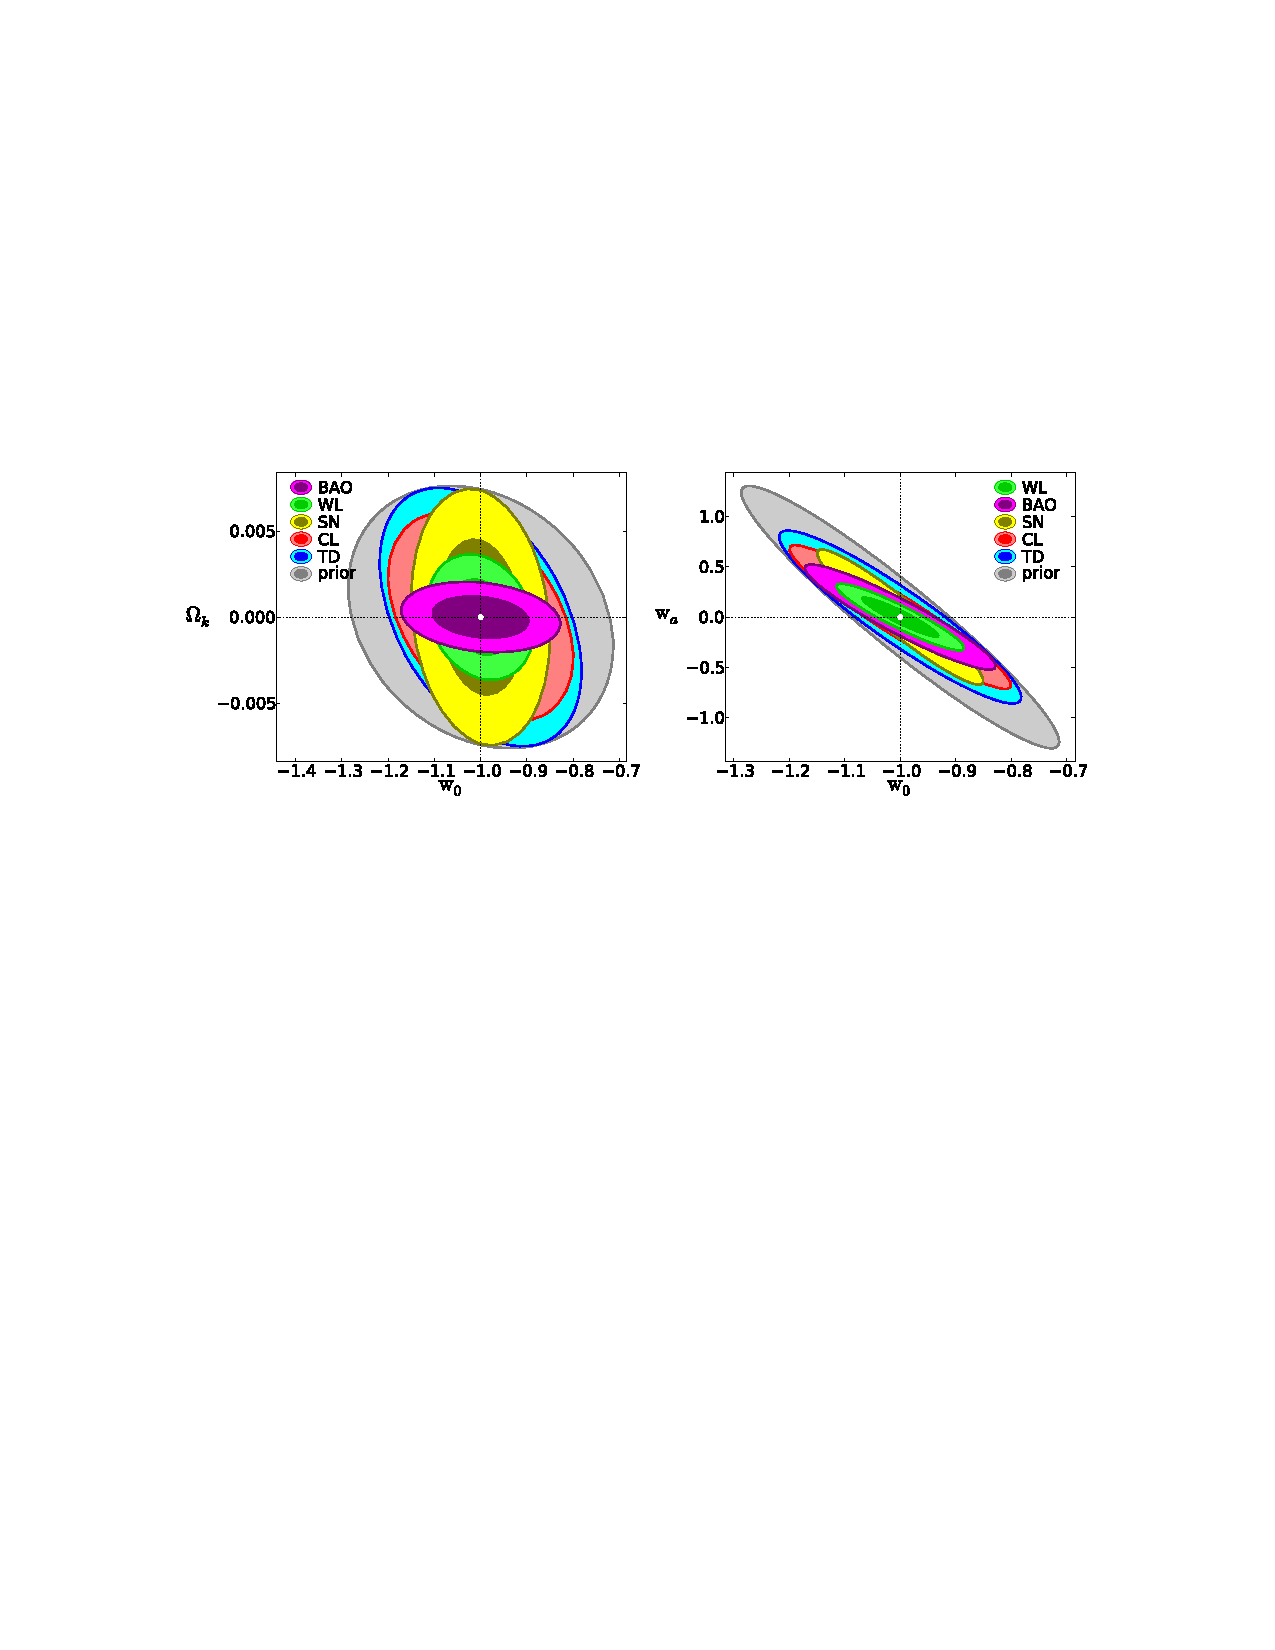
\includegraphics[width=0.9\linewidth]{figs/Coe+Moustakas2009_Figure14.pdf}
    \caption{LSST time delay lens cosmological parameter forecasts (blue)
    compared to optimistic forecasts from the Dark
    Energy Task Force (Albrecht et al 2006) for 4 other Stage IV probes.
    A sample of 100 lenses is assumed, each one
    providing a 5\% accurate time delay distance. Figure reproduced from
    Coe \& Moustakas (2009).}
    \label{fig:sl_forecast}
\end{figure*}

% ----------------------------------------------------------------------

\section{Experimental Design}
\label{sec:sl_design}

We now outline the proposed program's technology needs, introducing the
observations for each phase and describing the  instrumentation needed.

% ----------------------------------------------------------------------

\subsection{Detailed Mass Modeling to Enable Accurate Distance Determination}

To be useful as probes of cosmological distances, galaxy scale lenses
need very well constrained mass models. These constraints will come from
two sources:
\begin{enumerate}
    \item High resolution imaging of the Einstein rings due to the
    source AGN or SN host galaxy. Targeted snapshot (i.e.\ 200--2000
    second exposure time) imaging observations in the near infra-red
    with either JWST or a GSMT can provide the Einstein ring constraints
    needed to turn each of these systems into a  5\% precision distance
    (Meng et al 2015).
    \item Spatially resolved spectroscopy of the lens galaxy, enabling
    measurement of the stellar velocity dispersion field to break the
    degeneracy between the predicted time delays and the lens mass
    density profile, calibrating each system to enable it to provide a
    4\% accurate distance. We will need capabilities such as those
    currently available on Keck, and that will be available on all three
    of GMT, TMT and E-ELT (albeit with somewhat different technical
    specifications).
\end{enumerate}

However, before this we will need optical spectroscopy to get the
redshifts of the deflector and source galaxies. This can be done at
relatively low resolution, but the wider the wavelength range the
better: we will need 3500--10000 Angstroms in the optical, and maybe a
triplespec-like instrument covering the JHK bands in the IR. Some
redshifts may come from overlapping spectroscopic survey observations,
with the systems appearing as composite absorption and emission line
galaxy spectral components. Some of the targeted spectroscopy could be
done at 10-m class facilities.

After the redshift has been determined, AO-assisted integral field
spectroscopy would be best for providing the lens mass model constraints
(from both the Einstein rings and the spatially resolved spectroscopy).
We will need something like a 4"x4" field of view, with spectral
resolution R~4000--5000 over a wavelength range of 1.0--2.2 microns (to
cover CaT at rest frame  8800--9000A, or CO at 1.5-1.6$\mu$m). IRIS on
TMT would provide this capability, for example. OSIRIS on Keck is the
current best option, even though the field of view is a bit too small
and the current AO system at Keck has relatively low strehl at 1$\mu$m.
The Keck system will be upgraded, but TMT should be much better. Similar
data would be needed for the compound lenses.

While these targeted observations would be narrow field, they would
enable some considerable ancillary science, notably in the areas of
dark matter substructure (from perturbations to the imaged rings) and
AGN host galaxy structure.


% ----------------------------------------------------------------------

\subsection{Additional Monitoring of Selected Time Delay Systems}

If LSST's cadence is insufficient to provide Stage IV-accurate
measurements of lens time delays, we may need to supplement the light
curves with additional monitoring data. Most of the sample will have
lensed sources that are around 23rd magnitude in brightness, and so
monitoring will require dedicated scheduled imaging effort on 4--10m
class telescopes. For AGN, several year campaigns, with
weekly cadence interleaved with the LSST observations, would be needed.

Given the observational demands, smaller scale monitoring campaigns at
these depths may well be both desirable as well as feasible. High value
small sub-samples might include lensed type Ia supernovae, and variable
sources (i.e.\ AGN or supernovae) in compound lenses. The latter may
only occur in a handful of systems, but these highly constrained systems
would make valuable targets. Another possibility currently being
explored by Courbin et al, McCully et al, and others is to carry out
dedicated high cadence monitoring of lensed AGN, using the very short
time scale variability to probe the time delay more efficiently. If this
technique can be shown to work, it could reduce the demands on the
monitoring network considerably.

% ----------------------------------------------------------------------

\subsection{Multi-object Spectroscopy to Improve
the Fidelity of our Lens Environment and Line of Sight Characterization}

To achieve stage IV accuracy on cosmology, mass in the immediate
environment of the lens and along the line of sight cannot be ignored.
LSST will provide photometric redshifts and stellar masses of all
galaxies in the fields of each cosmographic lens. With this information,
following the methodology of Wong et al. 2011 and McCully et al. 2016,
we can remove the majority of the bias due to external convergence.
However, for some lens fields, this may not be enough; if there are
significant mass concentrations (e.g. clusters or groups), spectroscopy
may be required.

Multi-object spectroscopic data can provide significant improvements in
the accuracy of forward models. Spectroscopic coverage of the
$~5$~arcminute strong lens fields themselves is valuable, where many of
the benefits come from the redshifts of massive galaxies and groups
close to the line of sight. Based on mass models (that include some
spectroscopy), the uncertainty on the external convergence is a few
percent for an individual lens. However, spectroscopy can also provide
the velocity dispersion of both the lens galaxies and galaxies in the
lens environment or along the line of sight. The velocity dispersion of
the main lens galaxy allows us to break the lens radial profile
degeneracy, one of the key systematic uncertainties for measuring
cosmology using time delay cosmography. The velocity dispersion of the
environment/line of sight galaxies will allow more effective forward
modeling, further reducing the residual bias in external convergence
estimates by a factor of two (Collett et al. 2013). Characterization of
weak lensing effects for strong lensing has similar needs to that needed
to model intrinsic alignments.

DESI data is potentially valuable in the overlap region with LSST.
McCully et al. 2016 provide a method to rank order the contribution of
individual galaxies in the environment and along the line of sight. The
$\sim 30$ most important galaxies need to be modeled in full, making
them prime targets for spectroscopy, while the rest of the galaxies can
be approximated as with only shear and convergence, and likely only
require photometric data. By selecting only the most important galaxies
for spectroscopy, each lens field should only need a single pointing
from a Multi-object spectrograph, e.g. DESI, though fiber collisions may
necessitate multiple pointings. Spectroscopic training data for the
photometric redshifts and calibration fields could provide further
coverage.

% ----------------------------------------------------------------------

\section{Summary of Capabilities Required}
\label{sec:sl_summary}

{\bf Mass Modeling: Lens and Source Redshifts}: redshifts of the lens
and source are needed for an absolute lens mass measurement; the lens
redshift is needed to determine the set-up for follow-up stellar
kinematics measurement.

$\bullet$ Spectral coverage: as broad as possible, covering the range
between $u$ and $K$ bands.

$\bullet$ Spectral resolution: can be low, $R\sim1000$.

$\bullet$ Field of view: doesn't matter (targets are $\sim1$~arcsec in size),
but multi-object spectrograph covering at least a few arcmin is helpful,
to measure redshifts of other galaxies in the field.

$\bullet$ Proposed facilities: 10m-class telescopes for bright objects,
GSMTs for fainter systems.

$\bullet$ Total time required (100 systems): $\sim30$~hours, depending
on balance between facilities (assuming 20~mins per system, on average).



{\bf Mass Modeling: high resolution Einstein ring imaging}: this
constrains the mass model of the lens, including the density profile
slope (via the arc thickness).

$\bullet$ Spectral coverage and resolution: imaging in two or three bands is
recommended, to enable clean lens galaxy subtraction.

$\bullet$ Angular resolution: the higher the resolution the better, but
at least $0.1$~arcsec FWMH.

$\bullet$ Field of view: at least 4~arcsec, to capture the Einstein
ring without dithering.

$\bullet$ Proposed facilities: GSMTs, JWST. 10m-class telescopes for
brighter rings.

$\bullet$ Total time required: $\sim30$~hours, depending
on balance between facilities (assuming 20~mins per system, on average).


{\bf Mass Modeling: Spatially-resolved
Spectroscopy on Extremely Large Telescopes}: introduction.

$\bullet$ Spectral coverage and resolution: $R\approx4000-5000$  over a
wavelength range of 1.0--2.2 microns (to cover CaT at rest frame
$8800-9000\AA$, or CO at $1.5-1.6\mu$m).

$\bullet$ Angular resolution: 0.1--0.2~arcsec, to resolve the lens galaxy well.

$\bullet$ Field of view: at least 4~arcsec, to capture the lens galaxy
within the Einstein ring without dithering.

$\bullet$ Proposed facilities: GSMTs, JWST.

$\bullet$ Total time required: $\sim100$~hours, depending
on balance between facilities (assuming 60~mins per system, on average).


{\bf Additional Monitoring}: the working plan is not to need this, instead
just using the LSST light curves to measure time delays. However,
the LSST observing strategy might be chosen such that the time sampling
does not quite enable time delay measurement of sufficient accuracy for
cosmology; in this case, supplemental monitoring could make up the gap.

$\bullet$ Spectral coverage and resolution: could be single filter, $r$ or $i$. Other
bands may help with interpretation of LSST data.

$\bullet$ Angular resolution: $\sim1$~arcsec image quality or better.
Light curves of blended objects can be extracted by scene modeling,
where the best seeing LSST images drive the fit.

$\bullet$ Field of view: any.

$\bullet$ Proposed facilities: 2m, 4m or 8-10m class telescopes could
all play a role, as the lensed features being monitored will range in
mean brightness from 20 to 23 magnitudes.

$\bullet$ Total time required: matching the LSST coverage over five
seasons would mean some 450 visits, each of length a few minutes, for
each system (potentially all 100, but more likely a subset of the LSST
sample). Maximum cost: $\sim4000$~hours over five years  (some 80--100
nights per year). Minimum cost: $0$~hours, if LSST light curves are
found to be sufficient.

One of the main problems with this sort of monitoring campaign is the
scheduling: the only way it seems to be possible is with a dedicated
facility, perhaps one shared between a few different groups with similar
monitoring needs. The LSST transients and variables community presumably
have just such needs.


{\bf Environment characterization}: the primary goal here is redshift
determination of the galaxies in the lens fields, to improve the
fidelity of any mass reconstruction in those fields.

$\bullet$ Spectral coverage: as broad as possible, preferably $u$
through $K$.

$\bullet$ Spectral resolution: can be low, $R$ of a few hundred to a few
thousand.

$\bullet$ Field of view: at least 5~arcmin, preferably more.

$\bullet$ Proposed facilities: DESI, or similar multi-object spectrograph
on a 4m-class or bigger telescope.

$\bullet$ Total time required: $\sim100$~hours, assuming 1 hour per system.

There are significant gains to be made by combining these observations with
other redshift surveys, such as those for photometric redshift training
or calibration (Chapter~\ref{chp:photoz}).


% % ----------------------------------------------------------------------
%
% \subsection{Cluster Mass Function: Spectroscopic Surveying in Cluster Fields}
% \label{sec:sl:clusters}
% {\it Will Dawson and others}
%
% {\it Note from Will: While I have done a fair amount of cluster weak lensing and
% spectroscopy work, this has been focused on dark matter science, I am not
% actually an expert in cluster mass function cosmological constraints. That said
% I have drafted some text that I hope will describe the methods and needed
% capability (or capabilities) in enough detail that someone could determine
% whether they overlap with other needs. I am also includeing all spectroscopic
% cluster studies and those limited to strong lensing; we can move the text later
% if we like.}
%
% {\it Basic Premis}: Cosmology is sensitive to the abundance of rare massive
% clusters observed out to and beyond $z\sim 1$. For example, Takada \& Spergel
% (2014) have shown that a characterization of the most massive clusters can
% improve the constraining power of future cosmic shear surveys (e.g., LSST, and
% WFIRST) by approximately a factor of two, provided the cluster masses and
% redshifts are accurately constrained.
%
% Spectroscopy of cluster galaxies can improve LSST cluster mass function
% constraints in a number of ways:
% \begin{itemize}
%   \item {\it Redshifts of multiply imaged background galaxies}: Combined strong
%   and weak lensing measurements of clusters can improve both the cluster mass
%   and concentration constraints by approximately a factor of two (Umetsu et
%   al.~2010). So it is possible to improve the LSST cluster weak lensing
%   constraints by combining strong lensing measurement of the strongly lensed
%   background galaxies (preseumably identified from space-based observations,
%   such as HST or WFIRST, but potentially from LSST alone). However, redshifts of
%   the multiply lensed galaxies are needed in order to properly constrain the
%   cluster mass distribution. There has been some work recently by Keren Sharon's
%   group on the number of multiply lensed galaxy redshifts that are necessary for
%   a given lens model accuracy. Most of the multiply lensed galaxies are faint $R
%   \gtrsim 23$ and require large diameter telescopes.
%   \item {\it Accurate cluster redshifts}: For cosmological constraints it is
%   necessary to know both the mass and redshift of the clusters. While it is
%   possible to obtain better than average photometric redshifts of clusters due
%   to their being hundreds to thousands of galaxies to beat down the Poission
%   photo-z noise and the tight red sequence color relation, constaints can be
%   improved (how much) with accurate redshifts from spectroscopy. It is possible
%   to accomplish this with one to a few redshifts of the brightest cluster
%   galaxies. The instrument requirements are pretty relaxed for this science
%   since on only needs a few redshifts per pointing of rather bright galaxies.
%   \item {\it Cluster galaxy velocities as a probe of the cluster potential}: The
%   spectroscopic caustic method (Kaiser 1987; Regos \& Geller 1989) is the only
%   other successful stand alone method, in addition to weak lenising, of probing
%   the mass density profile to comparably large cluster radii. This is important
%   since joint CMB+SZE constraints indicate that SZE-derived {\em Planck} masses
%   underestimate the true $M_{500}$ masses by $b=1-\langle
%   M_{Planck}/M_\mathrm{true}\rangle\sim 43\%$ $\sim43\%$ --- far from the $\sim
%   20\%$ expected due to deviations from the influence of feedback, non-thermal
%   pressure, and cluster shapes (Battaglia+ 2012). Of even greater concern is
%   that according to WL studies (Sereno \& Ettori 2015), the bias appears to vary
%   with mass. SZE mass estimates are calibrated in part based on X-ray
%   temperatures with spectroscopy that is only reliable out to $r_{2500}\sim
%   0.25r_\mathrm{vir}$. Recent WL analyses of the {\em Planck} sample, that probe
%   the mass distribution to larger radii, yield $1-\langle
%   M_{Planck}/M_\mathrm{WL}\rangle\sim 30\%$ at the $\sim 10\%$ uncertainty level
%   (von der Linden+ 2014; Hoekstra+ 2015), somewhat relaxing the {\em Planck}
%   tension. Hinting at the importance of having probes of the cluster potential
%   out to large radii ($\sim$ the virial radius). To realize this science would
%   require more than a hundred spectroscopic redshifts per cluster, with a
%   moderate resolution spectrograph. A highly multiplexed moderate resolution
%   spectrograph, that can simulatinously target objects within $\lesssim
%   5$\,arcsecons of one another (due to the dense cluster environment). I (wd) am
%   not sure how many clusters would need to be surveyed to make a significant
%   improvement to planned LSST cluster cosmology.
%   \item {\it Redshift space distortions}: This is a probe of modified gravity,
%   and similar to the spectroscopic caustic method requires hundreds of
%   spectroscpic redshifts of cluster galaxies. The spectroscopic demands are the
%   same as the caustic method as well. I (wd) am not sure how many clusters we
%   would need to make this measurement for.
% \end{itemize}
%
% \ldots
%
% ======================================================================
